%\vspace*{-20mm}
%\centerline{\underline{\Large\bf Электромагнитный масс-сепаратор}}\vspace{5mm}
 
 \begin{picture}(190,85)(0,0)
 \put(10,0){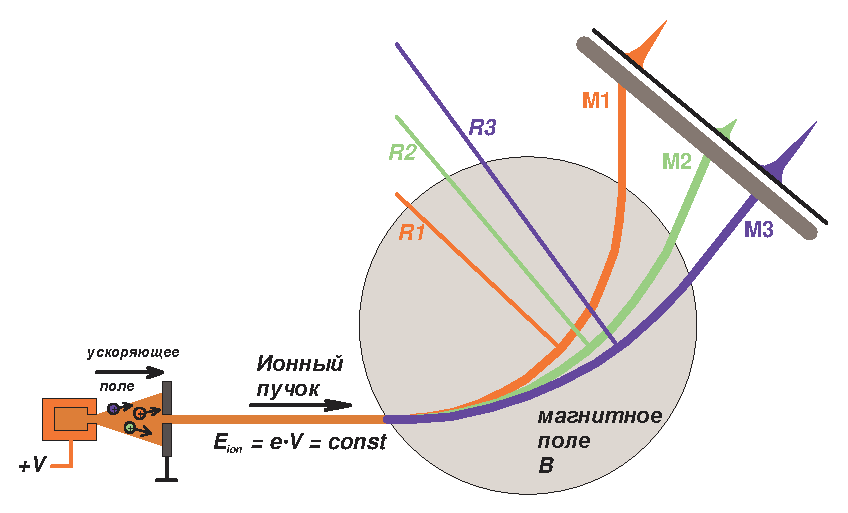
\includegraphics{GP019/GP019F01.eps}}
 \end{picture}\\[5mm]
\newpage
 \centerline{\Large\sl Oliver Heaviside (1850 - 1925) : \bf "импеданс"}
 \begin{picture}(190,60)(0,0)
 \put(0,0){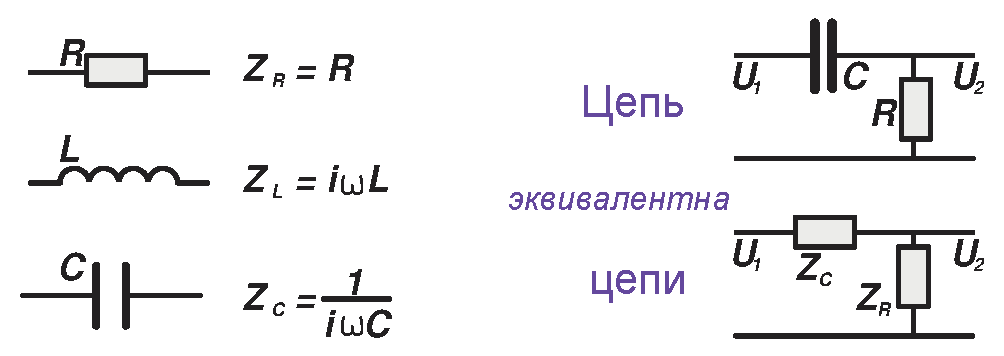
\includegraphics{GP019/GP019F02.eps}}
 \end{picture}\\[5mm]
Пусть входное напряжение $U_1$ -- это колебания с частотой $\omega$ и амплитудой $U_0$ :
\begin{displaymath}
U_1=U_0\;e^{i\omega t}
\end{displaymath}
требуется найти выходное напряжение $U_2(t)$ и ток $I(t)$. Для этого найдем импеданс всей цепи $Z$:
\begin{displaymath}
Z=Z_C+Z_R=\frac1{i\omega C}+R=R-\frac{i}{\omega C}=\frac{\omega CR-i}{\omega C}=|Z|\cdot e^{i\varphi}
\end{displaymath}\vspace{-3mm}
где \vspace{-3mm}
\begin{displaymath}
|Z|=\sqrt{\Re^2(Z)+\Im^2(Z)}=\sqrt{R^2+\frac1{(\omega C)^2}}=\left\{
\begin{array}{ll}
\infty&(\omega\rightarrow 0)\\
R\sqrt2&(\frac1{\omega C}=R)\\
R&(\omega\rightarrow\infty)
\end{array}\right.
;\hspace{5mm}\tan\varphi=\frac{\Im(Z)}{\Re(Z)}=\frac{-1}{\omega CR};\hspace{5mm}\varphi\in\left(-\frac\pi2\ldots0\right)
\end{displaymath}
Тогда ток в цепи равен\vspace{-3mm}
\begin{displaymath}
I=\frac{U_1}{Z}=\frac{U_0}{|Z|}\cdot \frac{e^{i\omega t}}{e^{i\varphi}}= |I_0|\cdot e^{i(\omega t-\varphi)}
\end{displaymath}
Определим теперь коэффициент передачи напряжения $k$ так, чтобы $U_2=k\cdot U_1$. Тогда
\begin{displaymath}
k=\frac{Z_R}{Z_C+Z_R}=\frac{R}{R+\frac1{i\omega C}}=\frac{i\omega CR}{1+i\omega CR}=
\frac{i\omega CR\;(1-i\omega CR)}{(1+i\omega CR)\;(1-i\omega CR)}=\frac{\omega CR\;(\omega CR+i)}{1+(\omega CR)^2}=|k|\cdot e^{i\psi}
\end{displaymath}
\begin{displaymath}
|k|=\frac{\omega CR\sqrt{(\omega CR)^2+1}}{1+(\omega CR)^2}=\frac{\omega CR}{\sqrt{1+(\omega CR)^2}}=\left\{
\begin{array}{ll}
\omega CR&(\omega\rightarrow 0)\\
1&(\omega\rightarrow\infty)
\end{array}\right.
;\hspace{5mm}\tan\psi=\frac{\Im(k)}{\Re(k)}=\frac{1}{\omega CR};\hspace{5mm}\psi\in\left(0\ldots\frac\pi2\right)
\end{displaymath}
Итак, после прохождения указанной цепи синусоида ослабнет по амплитуде в $|k|$ раз и будет немного опережать по фазе входное напряжение на угол $\psi$:
\begin{displaymath}
U_2=U_1\cdot k= U_1\cdot\frac{i\omega CR+(\omega CR)^2}{1+(\omega CR)^2}=U_0\;e^{i\omega t}\cdot|k|\;e^{i\psi}=\frac{U_0\;\omega CR}{\sqrt{1+(\omega CR)^2}}\cdot
e^{i(\omega t+\psi)}
\end{displaymath}
Так же можно поступать с электрическим сигналом \underline{\bf любой} формы. Для этого нужно разложить его на гармоники (в ряд Фурье), затем каждую из них домножить на $k$, и результаты снова сложить. Получим сигнал, прошедший через данную цепь.

Некоторые цепи имеют особое название:\\
 \begin{picture}(190,25)(0,0)
 \put(20,0){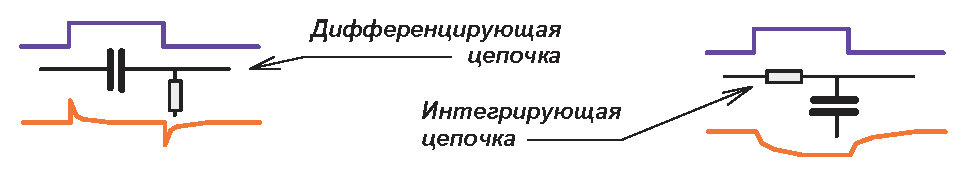
\includegraphics{GP019/GP019F03.eps}}
 \end{picture}\\
Действительно:
\begin{displaymath}
\frac{\partial U_1}{\partial t}=U_0i\omega\;e^{i\omega t}=U_1\cdot i\omega
\end{displaymath}
что при $\omega CR\ll1$ совпадает с $U_2$ в рассмотренном примере (с точностью до множителя $CR$=const).
